\providecommand{\main}{../../..}
\documentclass[\main/dresen_thesis.tex]{subfiles}

\begin{document}
  The solvent and co-solvent of the dispersion for the drop casting experiment determine the mobility of the nanoparticles and the time scales for the drop casting experiment.
  Early studies on drop casting of dodecanethiol-ligated gold nanospheres show that a combination of a toluene, a quickly evaporating solvent, as primary dispersion medium and dodecanethiol, a solvent with high-boiling point, as co-solvent results in long-range ordered nanostructure with spheres aligned on an hexagonal lattice \cite{Bigioni_2006_Kinet}.
  This idea has been transferred to oleic acid-ligated ferrite nanoparticles.
  The influence of the choice of primary/co-solvent mixture is studied by performing drop casting experiments using the nanocubes Ol-CoFe-C with varied alkane/alkene combinations.
  As alkane, n-pentane, n-hexane and n-heptane are chosen as rapidly evaporating component and for the high-boiling point alkene, 1-octadecene, 1-hexadecene, 1-dodecene, 1-decene and 1-tetradecene are studied.
  For every experiment the nanoparticle concentration of the dispersion is set to $0.13 \unit{mg/mL}$ and the co-solvent concentration to $2\unit{\%}$.
  Scanning electron microscopy is performed (\refapp{app:additionalExperimentalTechniques:sem}) for a first evaluation of the samples and to study the local order.
  For further quantification of the in-plane order, selected samples are measured using grazing incidence small-angle x-ray scattering at GALAXI under an incident angle of $\alpha_i \eq 0.11 \unit{^\circ}$ with a wavelength of $1.34 \unit{\angstrom}$.
  To quantify the thin layer structure, x-ray reflectometry was performed at the same instrument and wavelength by varying the incident angle in the range of $0\unit{^\circ} - 2\unit{^\circ}$ and measuring detector images for each angle.

  \begin{figure}[tb]
    \centering
    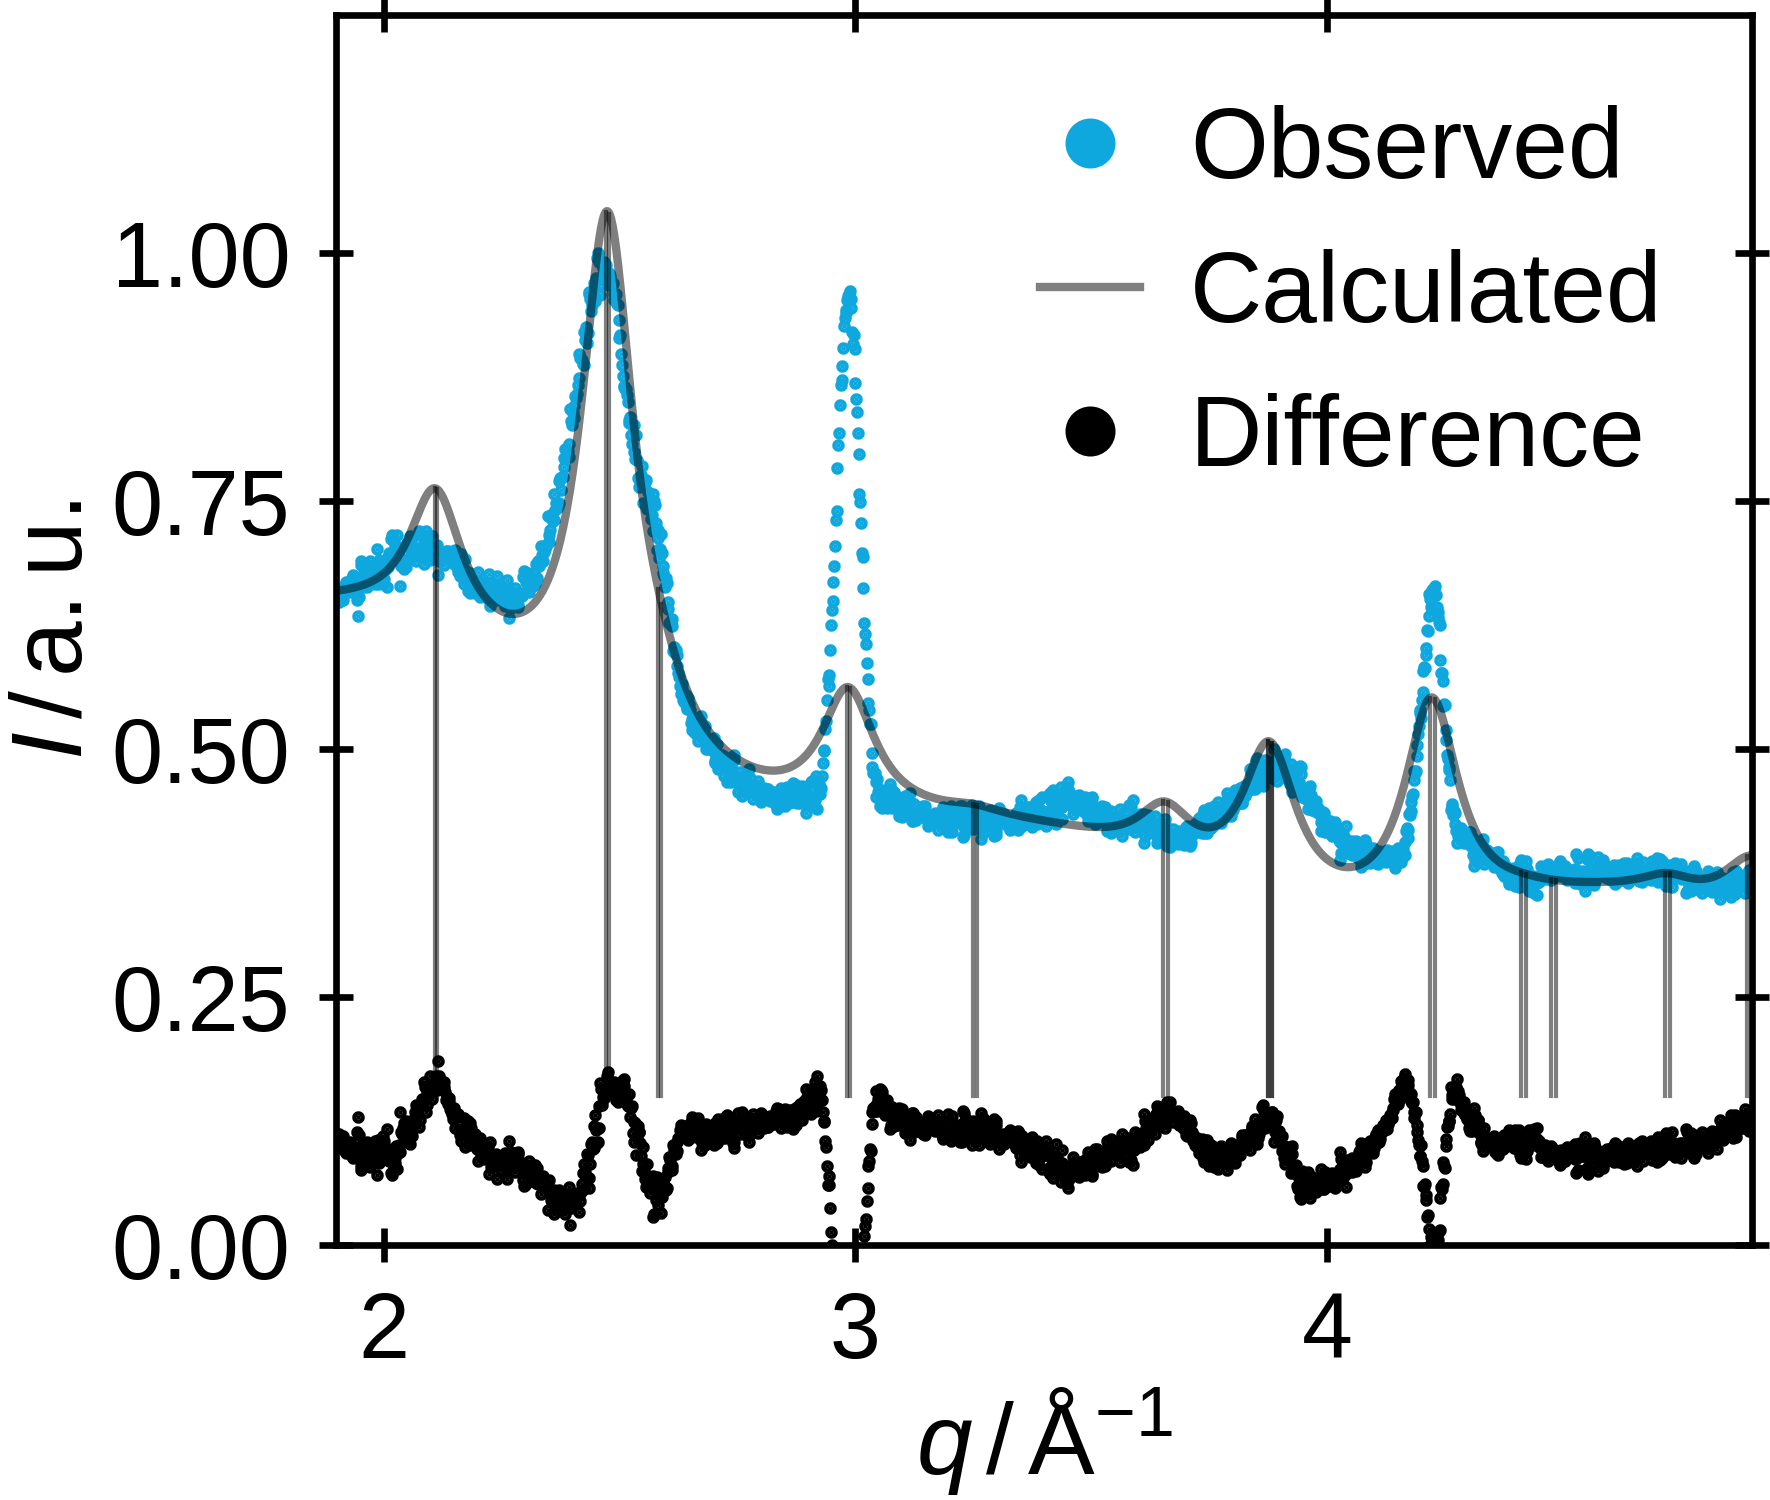
\includegraphics{monolayer_XRD_Ol_CoFe_C}
    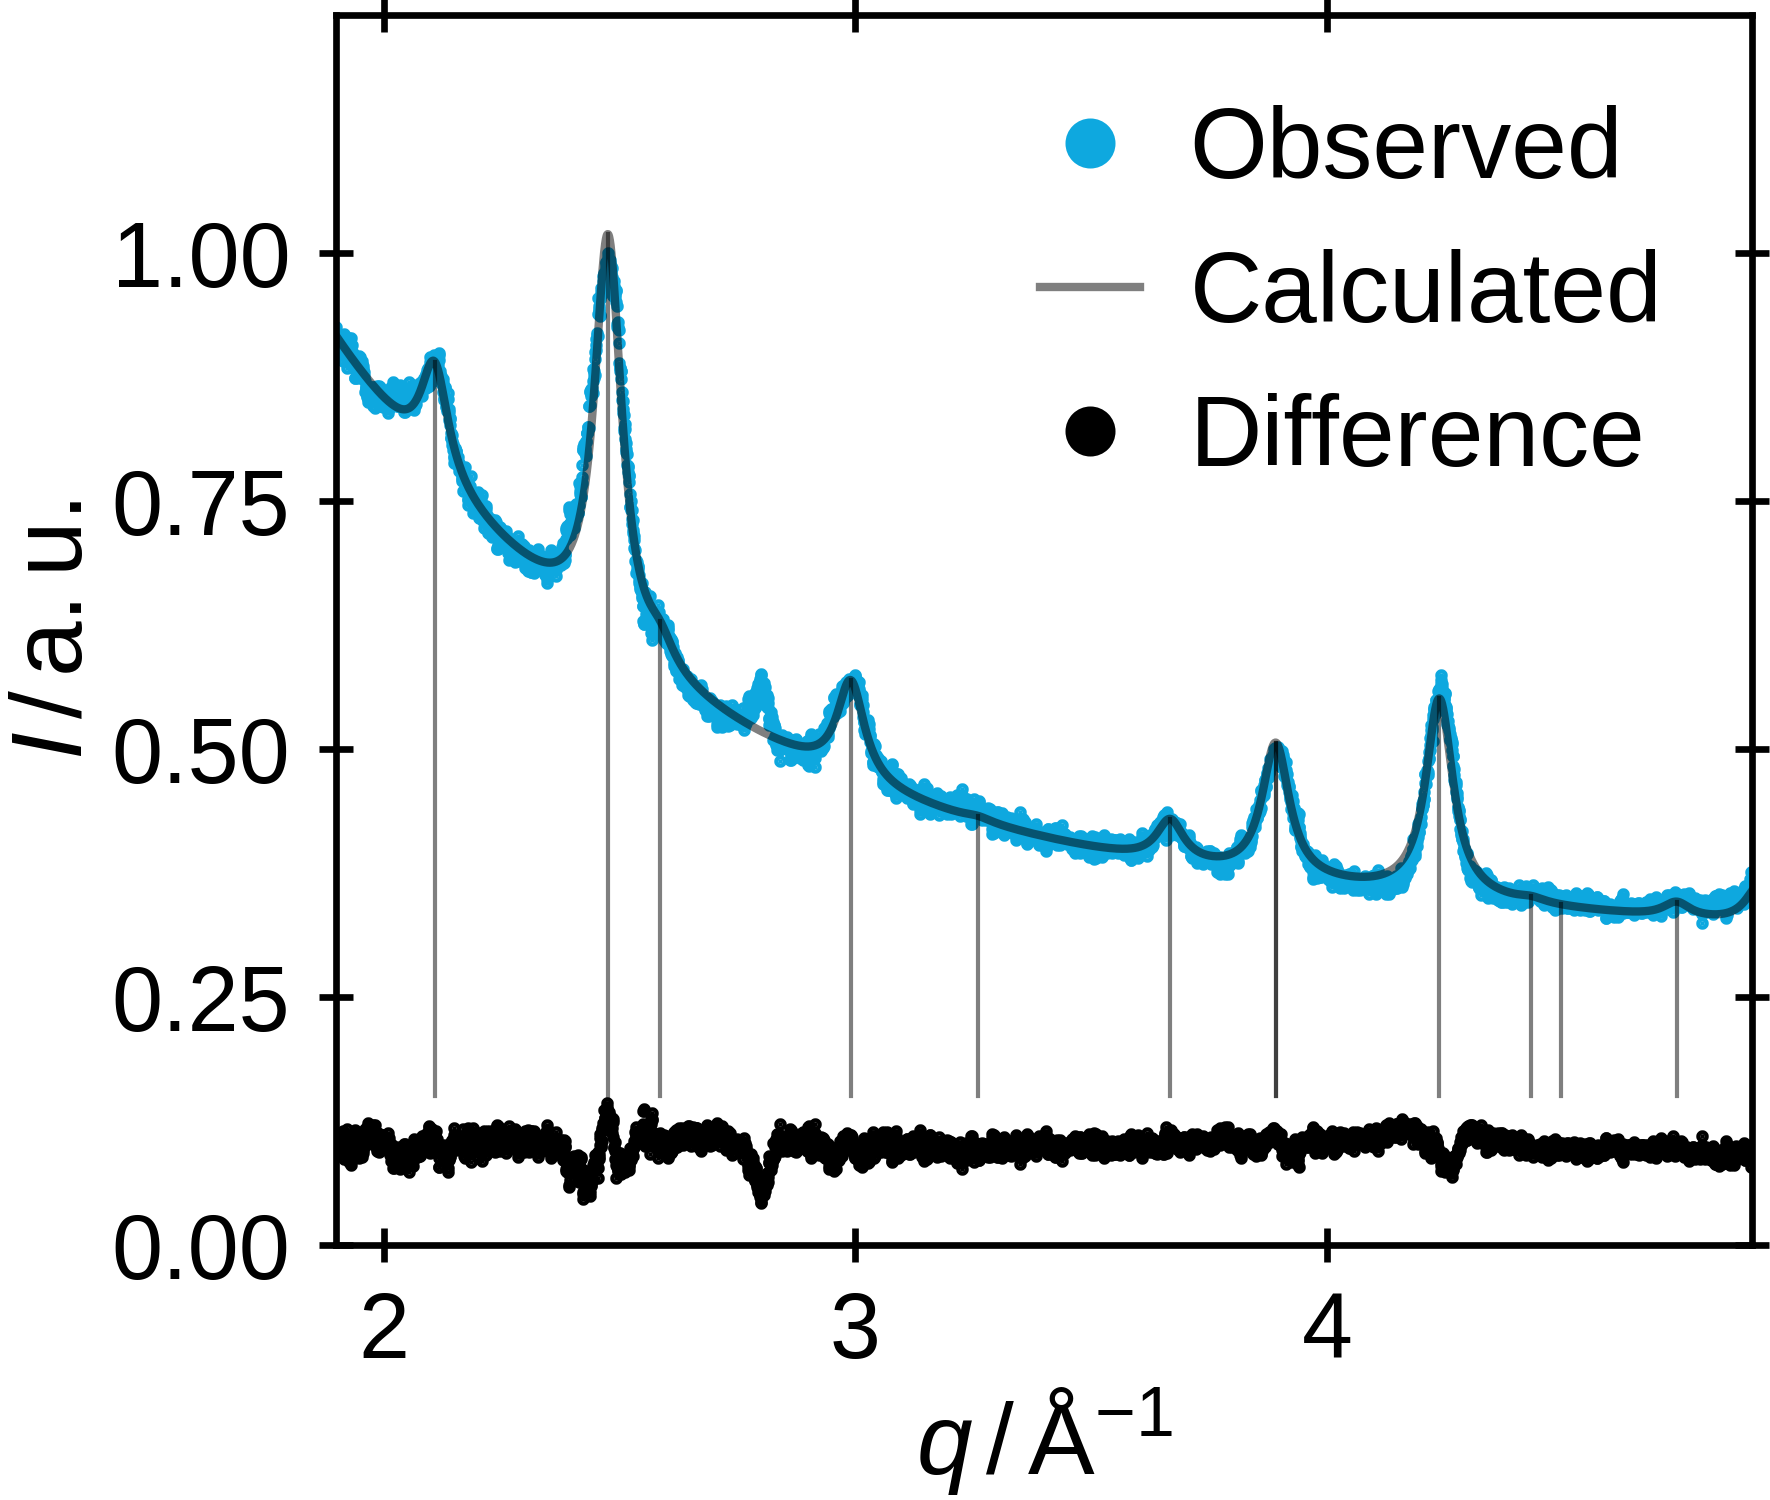
\includegraphics{monolayer_XRD_Ac_CoFe_C}
    \caption{\label{fig:monolayers:nanoparticle:xrd}X-ray diffraction of Ol-CoFe-C (left) and Ac-CoFe-C (right) with a Rietveld refinement assuming an inverse spinell structure.}
  \end{figure}


  The best quality of samples is achieved for a combination of n-heptane together with small addends of 1-octadecene and oleic acid as co-solvents.


  ...
  The concentration of the co-solvent...  

  
\end{document}